Das Ziel unserer Studie war es, zu überprüfen, ob die Interaktion zwischen Aufmerksamkeitsaktivierung und bewusster Aufmerksamkeitslenkung zu einer erhöhten räumlichen Aufmerksamkeit führt. Wir erweiterten dazu das vierte Experiment der Studie von \citeA{weinbach2012relationship} und manipulierten zusätzlich die Distanz der Flankierreize.
Wir haben erwartet, dass ein Ton die Abhnahme des Kongruenzeffekts mit der Distanz reduziert. Unsere Idee war es, dass, wenn sich der räumliche Fokus durch den Warnreiz weiten sollte, die Distraktoren auch bei größeren Abständen wahrgenommen werden würden und sich der Kongruenzeffekt daher weniger stark abschwächt.\\
\begin{figure*}[t]
	\centering
  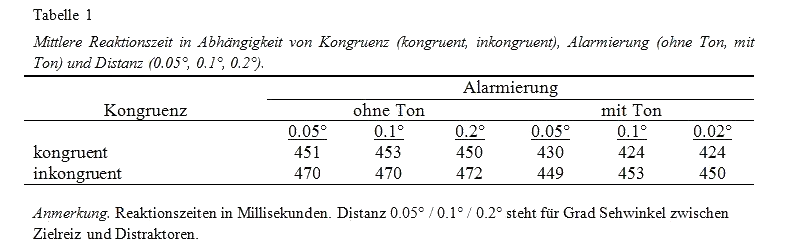
\includegraphics[width=\textwidth]{grafiken/Table-Kong_RT.png}
\end{figure*}
Diese Interaktion konnten wir nicht nachweisen. Ein möglicher Grund hierfür ist, dass wir unsere Distanzunterschiede mit 0.05°, 0.1° und 0.2° zu gering gewählt haben. Frühere Studien, welche eine Interaktion zwischen Distanz und Kongruenz nahe gelegt haben, verwendeten größere Distanzen \cite{eriksen1974effects}. Auch einen Haupteffekt für Distanz, wie ihn \citeA{eriksen1974effects} gefunden haben, konnten wir nicht finden. Dies ist möglicherweise ebenfalls auf die von uns verwendeten Distanzen zurückzuführen.\\
Auch die Ergebnisse des vierten Experiments von \citeA{weinbach2012relationship} konnten wir nicht vollständig replizieren. Es zeigten sich verkürzte Reaktionszeiten in den kongruenten Bedingungen, $F(1,22)=25.20$, $p<.001$, und in den Bedingungen mit Ton, $F(1,22)=29.17$, $p<.001$, was auch in Tabelle 1 dargestellt ist. Einen signifikanten Interaktionseffekt zwischen den beiden Faktoren, in unserem Experiment $F(1,22)=1.57$, $p=.22$, konnten wir nicht replizieren.
Eine Erklärung hierfür ist vermutlich unsere nicht exakte Replikation des Experiments, da wir dieses in einigen Punkten abgeändert haben. Zum einen verwendeten wir dunklerer Farben, welche zu einem schwereren Erkennen des Zielreizes geführt haben könnten. Es wäre also anzunehmen, dass unser Experiment schwieriger gewesen sein könnte und die mittleren Reaktionszeiten unserer Probanden daher langsamer gewesen wären. Die Analyse unserer Daten zeigte jedoch, dass die Reaktionszeiten mit denen der Probanden von \citeA{weinbach2012relationship} vergleichbar sind, wie in Abbildung~\ref{fig:vergleich} zu sehen ist.\\
Dies kann aber auch damit zusammenhängen, dass wir im Gegensatz zu \citeA{weinbach2012relationship} keine neutrale Bedingung in unserem Versuchsdesign hatten. Daraus folgt, dass die Trials mit inkongruenter Bedingung im Verhältnis zur Gesamtheit weniger werden und man daher seltener einen inkongruenten Trial erwartet. Es wäre daher anzunehmen, dass der Kongruenzeffekt in Experimenten mit neutraler Bedingung stärker ist.\\
Des Weiteren haben wir im Gegensatz zu \citeA{weinbach2012relationship} unsere Probanden in zwei Gruppen unterteilt, um beide Farb-Hand-Zuweisungen testen zu können. Jedoch zeigten auch die Einzelauswertungen nach Farb-Hand-Zuweisung keine nennenswerten Unterschiede zur Gesamtauswertung.\\
\begin{figure}[t]
	\centering
		\begin{subfigure}[b]{0.49\textwidth}
	       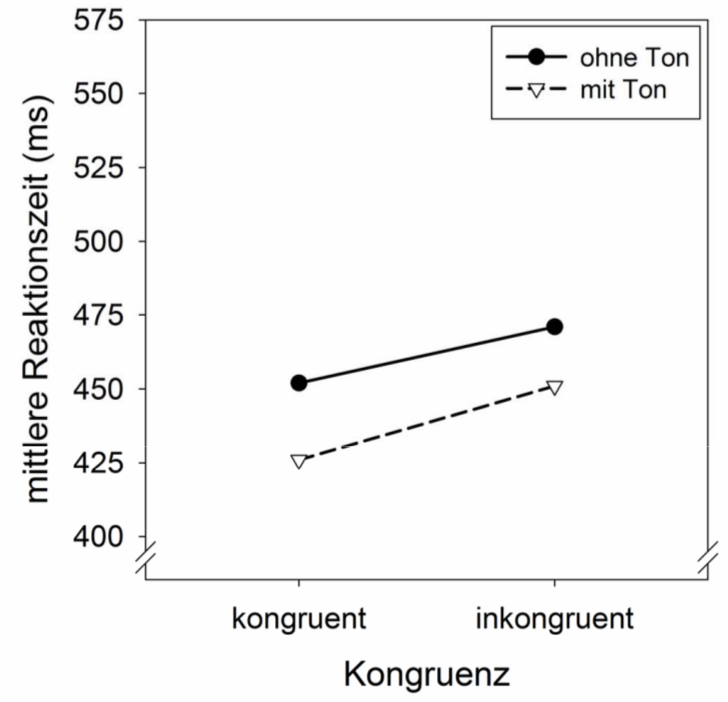
\includegraphics[width=\textwidth]{grafiken/Vergleich-unser.png}
	       \caption{Unser Experiment}
	       \label{fig:exp1}
	    \end{subfigure}%
	       ~
	    \begin{subfigure}[b]{0.49\textwidth}
	       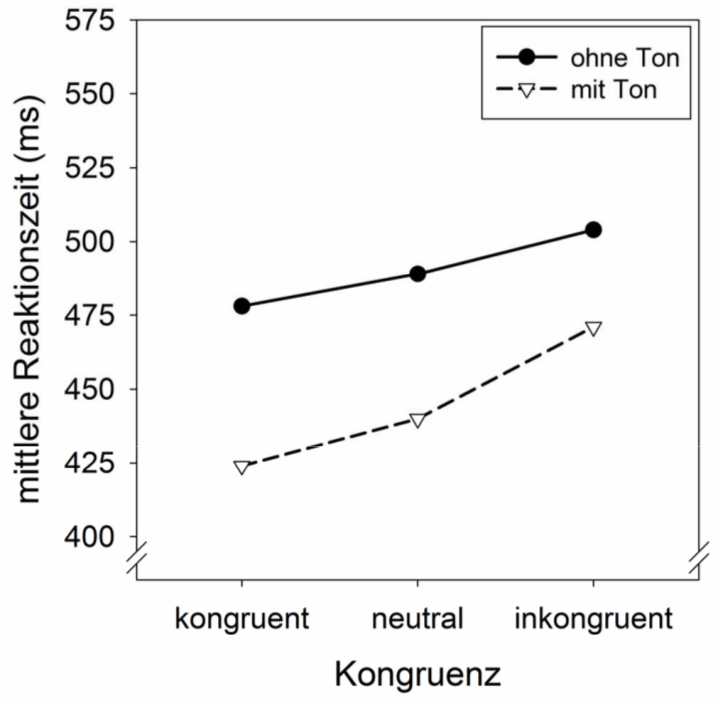
\includegraphics[width=\textwidth]{grafiken/Vergleich-henik.png}
	       \caption{Henik und Weinbach (2012)}
	       \label{fig:exp2}
	    \end{subfigure}
		\caption{Mittlere Reaktionszeiten im Vergleich}
		\label{fig:vergleich} 
\end{figure}
Evidenz für unser Hypothese konnten wir aus den zuvor genannten Gründen nicht nachweisen. Die Probleme, welche unserem Versuchsaufbau zu Grunde liegen, lassen sich jedoch leicht vermeiden. In einem möglichen Nachfolgeexperiment sollten die Distanzunterschiede vergrößert werden. Eine mögliche Größe der Distanzunterschiede könnten die bereits von \citeA{eriksen1974effects} erfolgreich verwendeten Abstände von 0.06°, 0.5° und 1° sein.\\
Da wir auch den Interaktionseffekt aus dem Experiment von \citeA{weinbach2012relationship} nicht replizieren konnten, sollte man, bevor man weitere Untersuchungen in Betracht zieht, ihr Experiment vollständig replizieren. Hierbei könnte man auch testen, wie sich die Interaktion bei anderen Distraktoren verhält. Als mögliche andere Distraktorreize könnte man die Buchstaben, welche \citeA{eriksen1974effects} in ihrer Untersuchung verwendeten, benutzen. Anschließend wäre eine Wiederholung unseres Experiments mit vergrößerten Distanzen und einer neutralen Bedingung möglich, um die Fehler aus unserer Untersuchung zu vermeiden.\\
Die Mechanismen, die unserer Aufmerksamkeitaktivierung zu Grunde liegen, benötigen weitere Untersuchungen, um unser Wissen über eine unserer zentralen kognitiven Fähigkeiten, der Aufmerksamkeit, zu erweitern. Obwohl wir mit unserer Studie nur wenig neue Erkenntnisse zu diesem spannenden Thema sammeln konnten, liefert unsere Untersuchung Erkenntnisse, die helfen können, die von uns gemachten Fehler in zukünftigen Studien zu vermeiden. 
